% ==================///==================///==================///
% ==================/// LATEX'S STUFF
% ==================///==================///==================///

\documentclass[hungarian]{beamer}
\usepackage[T1]{fontenc}
\usepackage{babel}
\usepackage{graphicx}
\usepackage{hyperref}
\usepackage{stuki}

\usepackage{amsfonts,amsmath,oldgerm}
\usetheme{_statale}
\usefonttheme[onlymath]{serif}

\newcommand{\testcolor}[1]{\colorbox{#1}{\textcolor{#1}{test}}~\texttt{#1}}
\newcommand{\hrefcol}[2]{\textcolor{cyan}{\href{#1}{#2}}}
\titlebackground*{assets/background}

\newcommand{\Ord}{\mathcal{O}}


% ==================///==================///==================///
% ==================/// SPLASH PAGE
% ==================///==================///==================///

\title{Algoritmusok I.}
\newcommand{\longauthor}{2. gyakorlat}
\author{Sipos Ágoston}
\newcommand{\correspondingauthor}{John Doe}
\newcommand{\email}{siposagoston@inf.elte.hu}
\renewcommand{\insertdate}{2026. szeptember 16.}

% ==================///==================///==================///
% ==================/// START PRESENTATION
% ==================///==================///==================///

\begin{document}
\maketitle

\section{Aszimptotika}

\begin{frame}{Emlékeztető}

Múlt héten láttuk néhány algoritmus aszimptotikus költségét:
\begin{itemize}
    \item Polinom kiértékelése $\mathcal{O}(n)$
    \item Buborékrendezés, max.kiv. rendezés $\mathcal{O}(n^2)$
\end{itemize}

Mik a gyakran előforduló műveletigények, és melyik a gyorsabb közülük?
    
\end{frame}

\begin{frame}{Gyakori függvényosztályok}
\begin{itemize}
    \item Polinomiális: $\Ord(n)$, $\Ord(n^2)$, \dots, $\Ord(n^k)$ ($k \in \mathbb{Z^+}$)
    \begin{itemize}
        \item Gyökös, egyéb törtkitevős hatvány: $\Ord(\sqrt{n})$, $\Ord(n^r)$ ($r \in \mathbb{R}^+$)
    \end{itemize}
    \item Logaritmus: $\Ord(\log n)$ Pl. bináris keresés
    \item Konstans, jele: $\Ord(1)$ Pl. tömb elérése indexszel
    \item Exponenciális: $\Ord(2^n)$, $\Ord(3^n)$, \dots Pl. Fibonacci ügyetlenül megírva, egy halmaz összes részhalmazának felsorolása
    \item Faktoriális: $\Ord(n!)$ Pl. tömb összes permutációjának előállítása
\end{itemize}
\end{frame}

\begin{frame}{Relációk}
\begin{itemize}
    \item $\Ord(n!) > \Ord(a^n)$ (bármely $a>1$)
    \item $\Ord(a^n) > \Ord(b^n)$, ha $a > b$
    \item $\Ord(a^n) > \Ord(n^k)$ (bármely $a>1$ és $k > 0$)
    \item $\Ord(n^k) > \Ord(n^l)$, ha $k > l$
    \item $\Ord(n^k) > \Ord(\log_b n)$ (bármely $k > 0$ és $b > 1$)
    \item $\Ord(\log_b n) = \Ord(\log_c n)$ (bármely $b, c > 1$)
    \item $\Ord(\log_b n) > \Ord(1)$
\end{itemize}

Több tagból álló kifejezések esetén elég a legnagyobbat figyelembe venni, az ,,dominál''

\end{frame}

\begin{frame}[t]{Példa}

Tegyük aszimptotikus műveletigény szerint növekvő sorba:

$n! + n^2$; \qquad $n \cdot \log_2 n$; \qquad $n \cdot \sqrt{n} + 2 n^{\frac{3}{2}}$; \qquad $\log_{10} (n^3)$; \qquad $e^n$
    
\end{frame}

\section{Verem}

\begin{frame}{Szemléltető ábra}

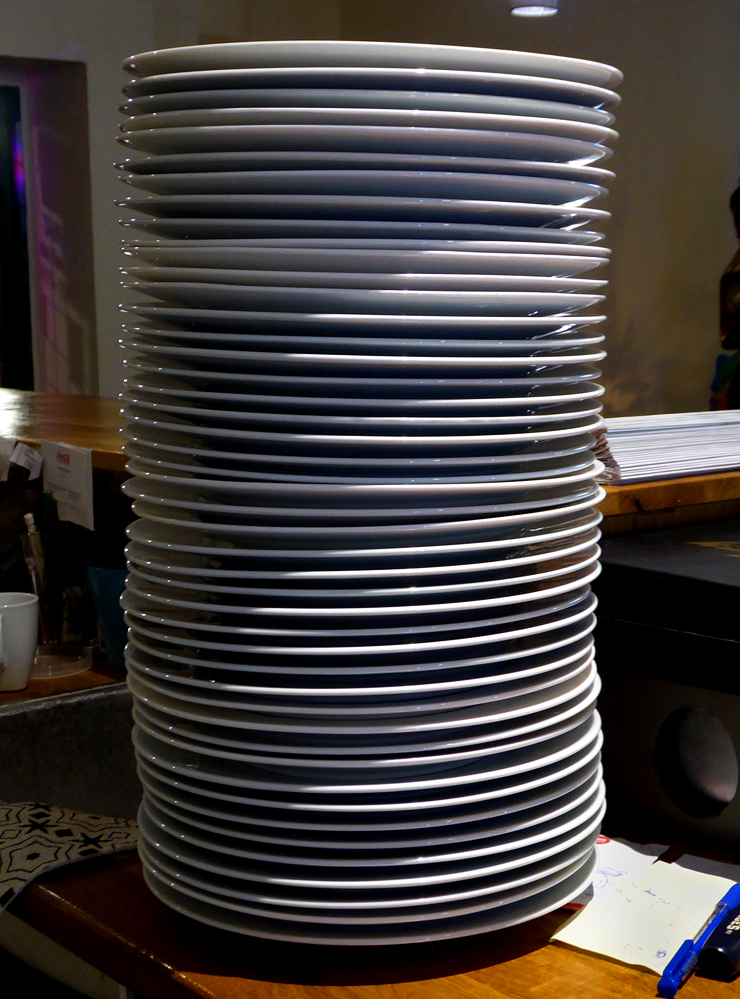
\includegraphics[width=0.3\linewidth]{assets/image.png}\hfill
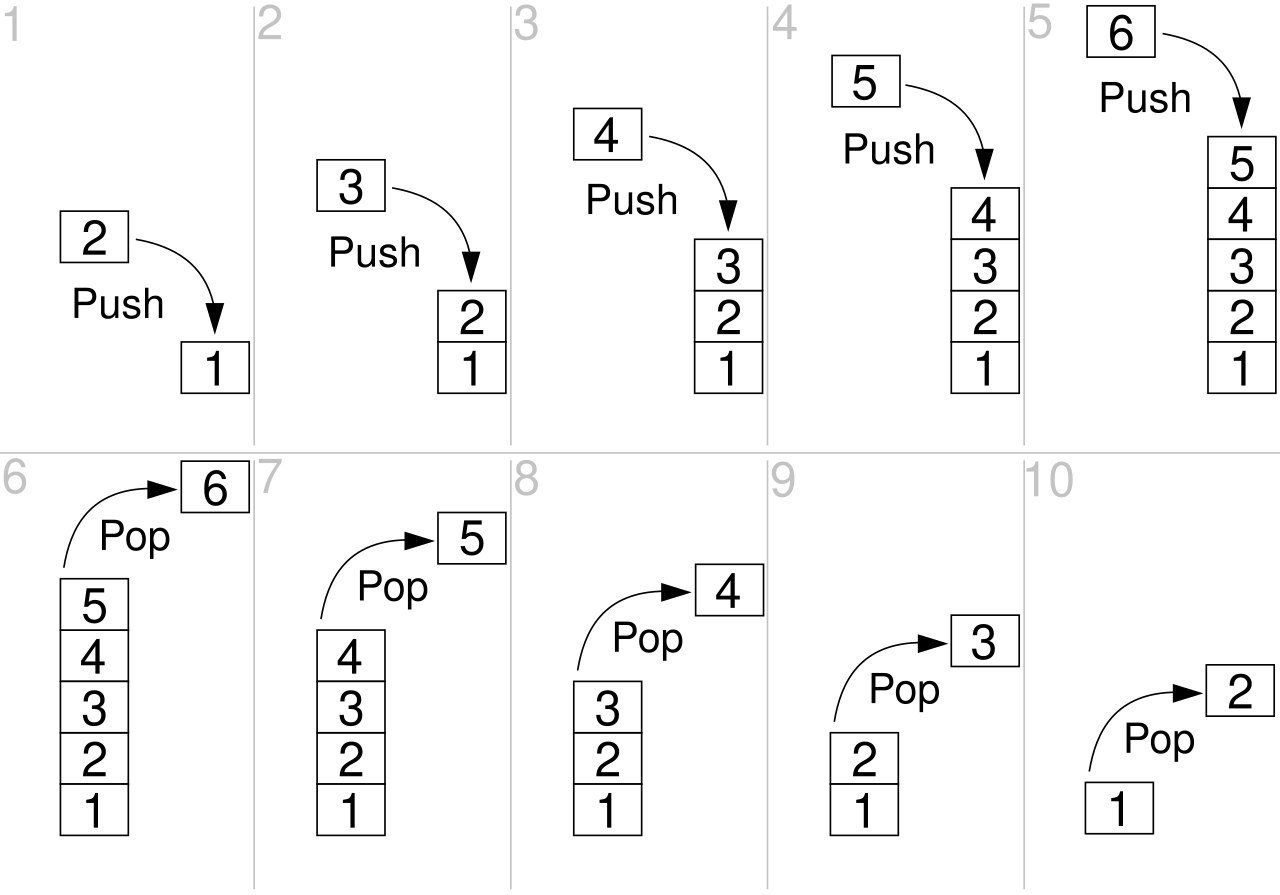
\includegraphics[width=0.5\linewidth]{assets/lifo.png}

\end{frame}

\begin{frame}{Verem / Stack absztrakt adattípus}

Műveletek:

Stack() -- létrehoz egy üres vermet

push(x : T) -- az x elemet a verem tetejére teszi

pop(): T -- a verem legfelső elemét eltávolítja, és visszaadja

top(): T -- a verem legfelső elemét visszaadja

isEmpty(): $\mathbb{B}$ -- visszaadja, hogy van-e elem a veremben

\vspace{6mm}

\begin{itemize}
    \item Hogyan megvalósítható?
    \item Hogyan használható?
\end{itemize}

A két kérdés teljesen külön kezelhető (enkapszuláció, fekete doboz)

Persze célszerű tudni a műveletek műveletigényét...

\end{frame}

\begin{frame}[t]{Verem megvalósítása fix méretű tömbbel}

Reprezentáció: t : T[m] (1-től indexelt), n : integer (csak addig működik, amíg $n \leq m$)

Minden művelet legyen $\Ord(1)$


\noindent\hfill
\begin{stukibox*}[3cm]{Stack()}\stm*{n = 0}\end{stukibox*}%
\hfill
\begin{stukibox*}[3cm]{top()}\stm*{return t[n]}\end{stukibox*}%
\hfill
\begin{stukibox*}[3cm]{isEmpty()}\stm*{return n > 0}\end{stukibox*}%
\hfill{}

\vspace{5mm}

\noindent\hfill
\begin{stukibox*}[3cm]{pop()}\stm*{x = t[n]}\stm*{n = n - 1}\stm*{return x}\end{stukibox*}%
\hfill
\begin{stukibox*}[3cm]{push(x)}\stm*{n = n + 1}\stm*{t[n] = x}\end{stukibox*}%
\hfill{}

\end{frame}

\begin{frame}{Példa - tömb megfordítása veremmel}

Bemenet: a : T[n]

\setlength{\stukiwidth}{4cm}
\newcommand{\oneton}{1\,\textrm{to}\,n}
\begin{stukibox}
\stm*{s = Stack()}
\begin{WHILE}{2}{\stm{i = \oneton}}
\stm*{s.push(a[i])}
\end{WHILE}
\begin{WHILE}{2}{\stm{i = \oneton}}
\stm*{a[i] = s.pop()}
\end{WHILE}
\end{stukibox}

\end{frame}

\begin{frame}[t]{Zárójelpárok}

Keressük meg egy csukó zárójel nyitó párját a szövegben. (Pl. syntax highlighting)

\only<1>{Először: helyes-e a zárójelezés?}

\only<2>{Ötlet: tegyük a nyitó zárójelek helyét a verembe. Ha minden csukó zárójelnél kivesszük a legfelső elemet, akkor mindig az adott zárójel párját vesszük ki.

Bemenet: s : string (a teljes szöveg), k : integer (a csukó zárójelünk indexe)}

\end{frame}

\begin{frame}{Szorgalmi -- Tükrözött szöveg}
Tükrözött-e a szöveg? Adott egy legfeljebb m hosszú,
betűkből és ’\#’ szimbólumokból álló sorozat. A sorozatot
tükrözöttnek nevezzük, ha felbontható olyan páratlan
hosszú, palindrom karaktersorozatokból álló részekre,
melyek középső karaktere egy ’\#’ karakter. Egyszer végig
olvasva a szöveget döntsük el, hogy tükrözött-e? Az
algoritmus egyetlen vermet, és egyszerű segédváltozókat
használhat.

Példa:

Tükrözött: \#, \#\#\#\#, abc\#cba, \#\#a\#aabc\#cba

Nemtükrözött: abc, abc\#cb, abc\#cbaa\#aa, ab\#bac\#\#c

\end{frame}

\section{Posztfix jelölés (Fordított lengyel forma / RPN)}

\begin{frame}{Fordított Lengyel Forma}
Lengyel forma: egy aritmetikai kifejezés postfix alakja.

Például:
$1+2 * 3 \rightarrow 1\;2\; 3 * +$

$(1+2) * 3 \rightarrow 1\; 2 + 3\;*$

Jellemzői:
\begin{itemize}
    \item Nincsenek benne zárójelek, a kiértékelés mégis egyértelmű,
és könnyen elvégezhető.
    \begin{itemize}
        \item ,,Láthatatlan'' zárójelek: $(1\;(2\;3\;*)\;+)$, ill. $((1\; 2\; +)\;3\;*)$
    \end{itemize}
    \item Operandusok sorrendje nem változik, az infix kifejezéshez
képest.
    \item Operátorok sorrendje: az elvégzésük sorrendjében
szerepelnek.
    \item Minden operátort közvetlen megelőznek az operandusai,
tehát amikor egy operátor megjelenik, biztosan az előtte
lévő operandusokra vonatkozik.
    \item Az operandus lehet változó, konstans, de lehet postfix
kifejezés is.
\end{itemize}
\end{frame}

\begin{frame}{RPN kiértékelése}

Veremmel. Ha konstans jön, a verembe tesszük. Ha operandus, kivesszük a két felsőt, végrehajtjuk a műveletet, az eredményt a verembe tesszük.

\newcommand{\oneton}{1\,\textrm{to}\,n}
\begin{stukibox}
\stm{s = Stack()}
\begin{WHILE}{5}{\stm{!inp.eof()}}
\stm{a = inp.read()}
\begin{IF}{3}{\stm*{$a$ is an operator}}
\stm{r = s.pop()}
\stm{b = eval(s.pop(), a, r)}
\stm{s.push(b)}
\ELSE
\stm{s.push(a)}
\end{IF}
\end{WHILE}
\stm*{return $s.pop()$}
\end{stukibox}
(Utófeltétel: a verem üres!)
\end{frame}

\begin{frame}[t]{RPN kiértékelése -- példa}

8 2 + 3 2 \textasciicircum \,* 5 15 - /

\end{frame}

\begin{frame}{RPN előállítása}

\begin{figure}
    \centering
    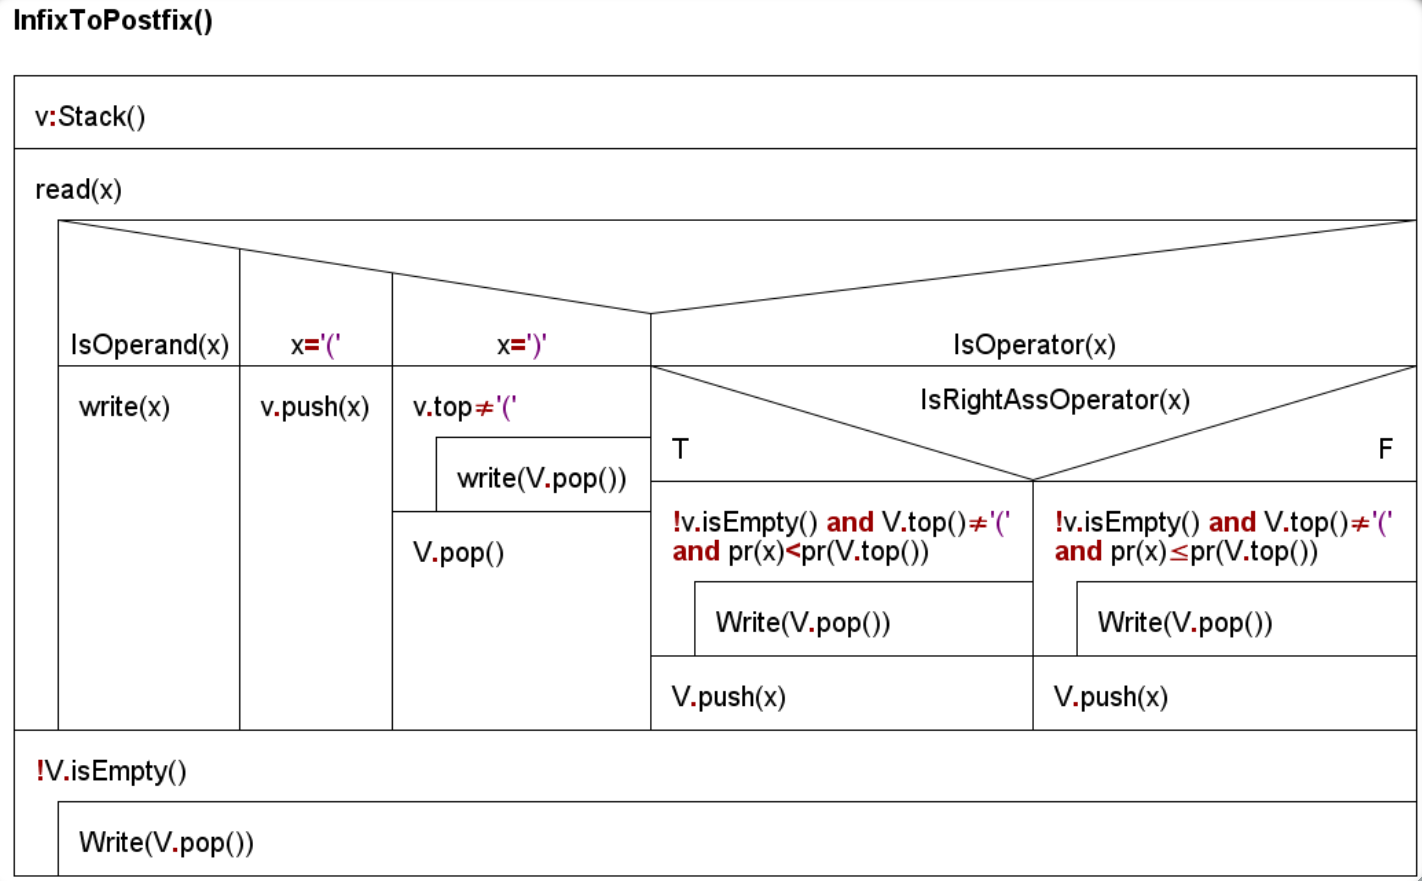
\includegraphics[width=0.7\linewidth]{assets/shuntingyard.png}
\end{figure}

\end{frame}

\begin{frame}[t]{RPN előállítása -- példa}

\begin{columns}[T]
\begin{column}{0.5\linewidth}
    \centering
    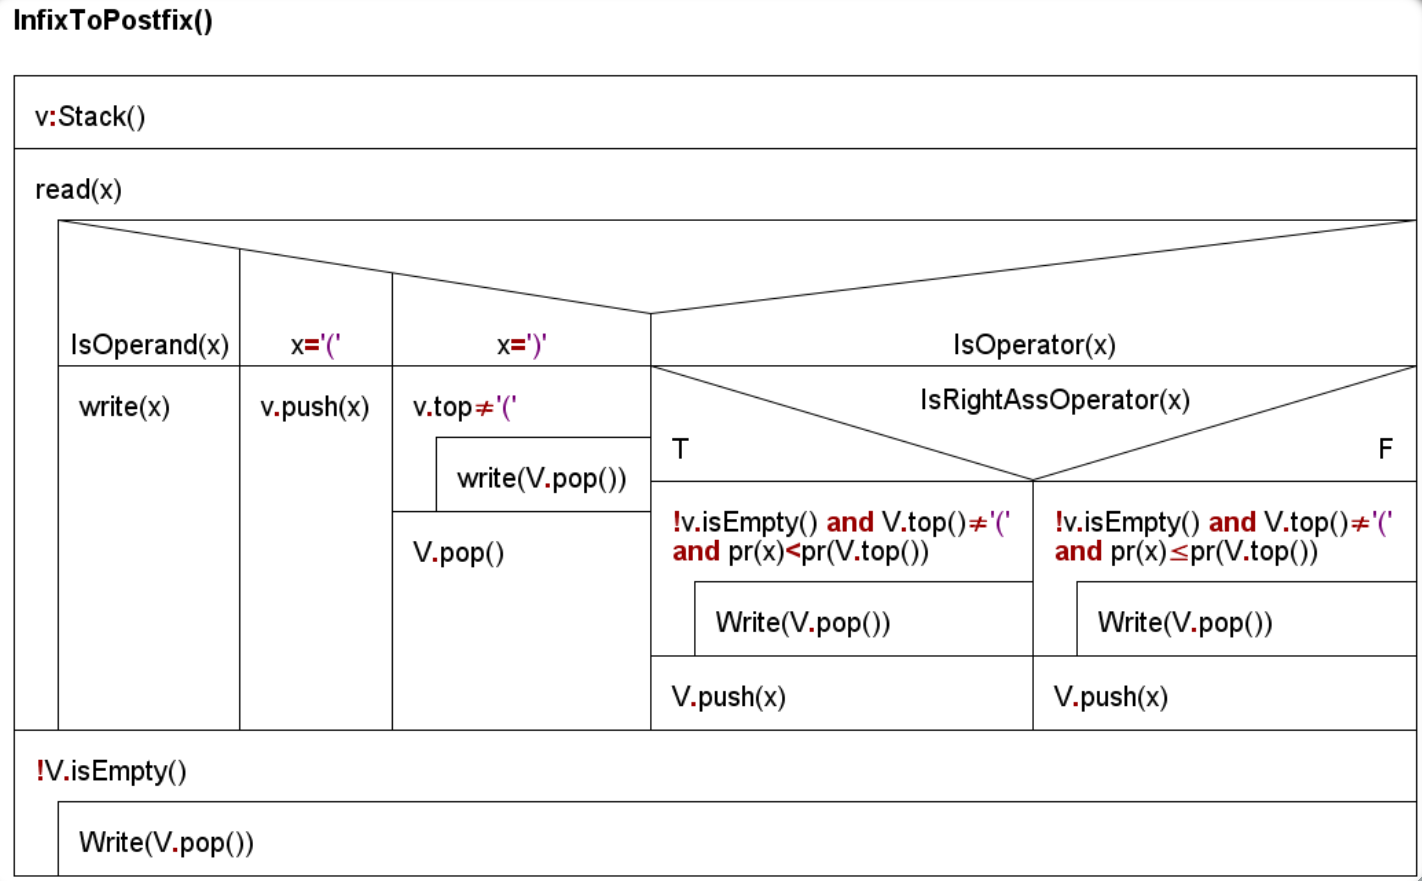
\includegraphics[width=\linewidth]{assets/shuntingyard.png}
\end{column}
\begin{column}{0.5\linewidth}
    Bemenet: b + 2 / (a - c) - (f \textasciicircum \,b \textasciicircum \,2 * g) / z + w
\end{column}

\end{columns}

\end{frame}

\iffalse
\section{Sor}

\begin{frame}{Sor}

Nagyon hasonló a veremhez, analóg műveletek, annyi a különbség, hogy az új elemet a sor végére rakjuk; tehát az van a sor elején, ami legkorábban került be.

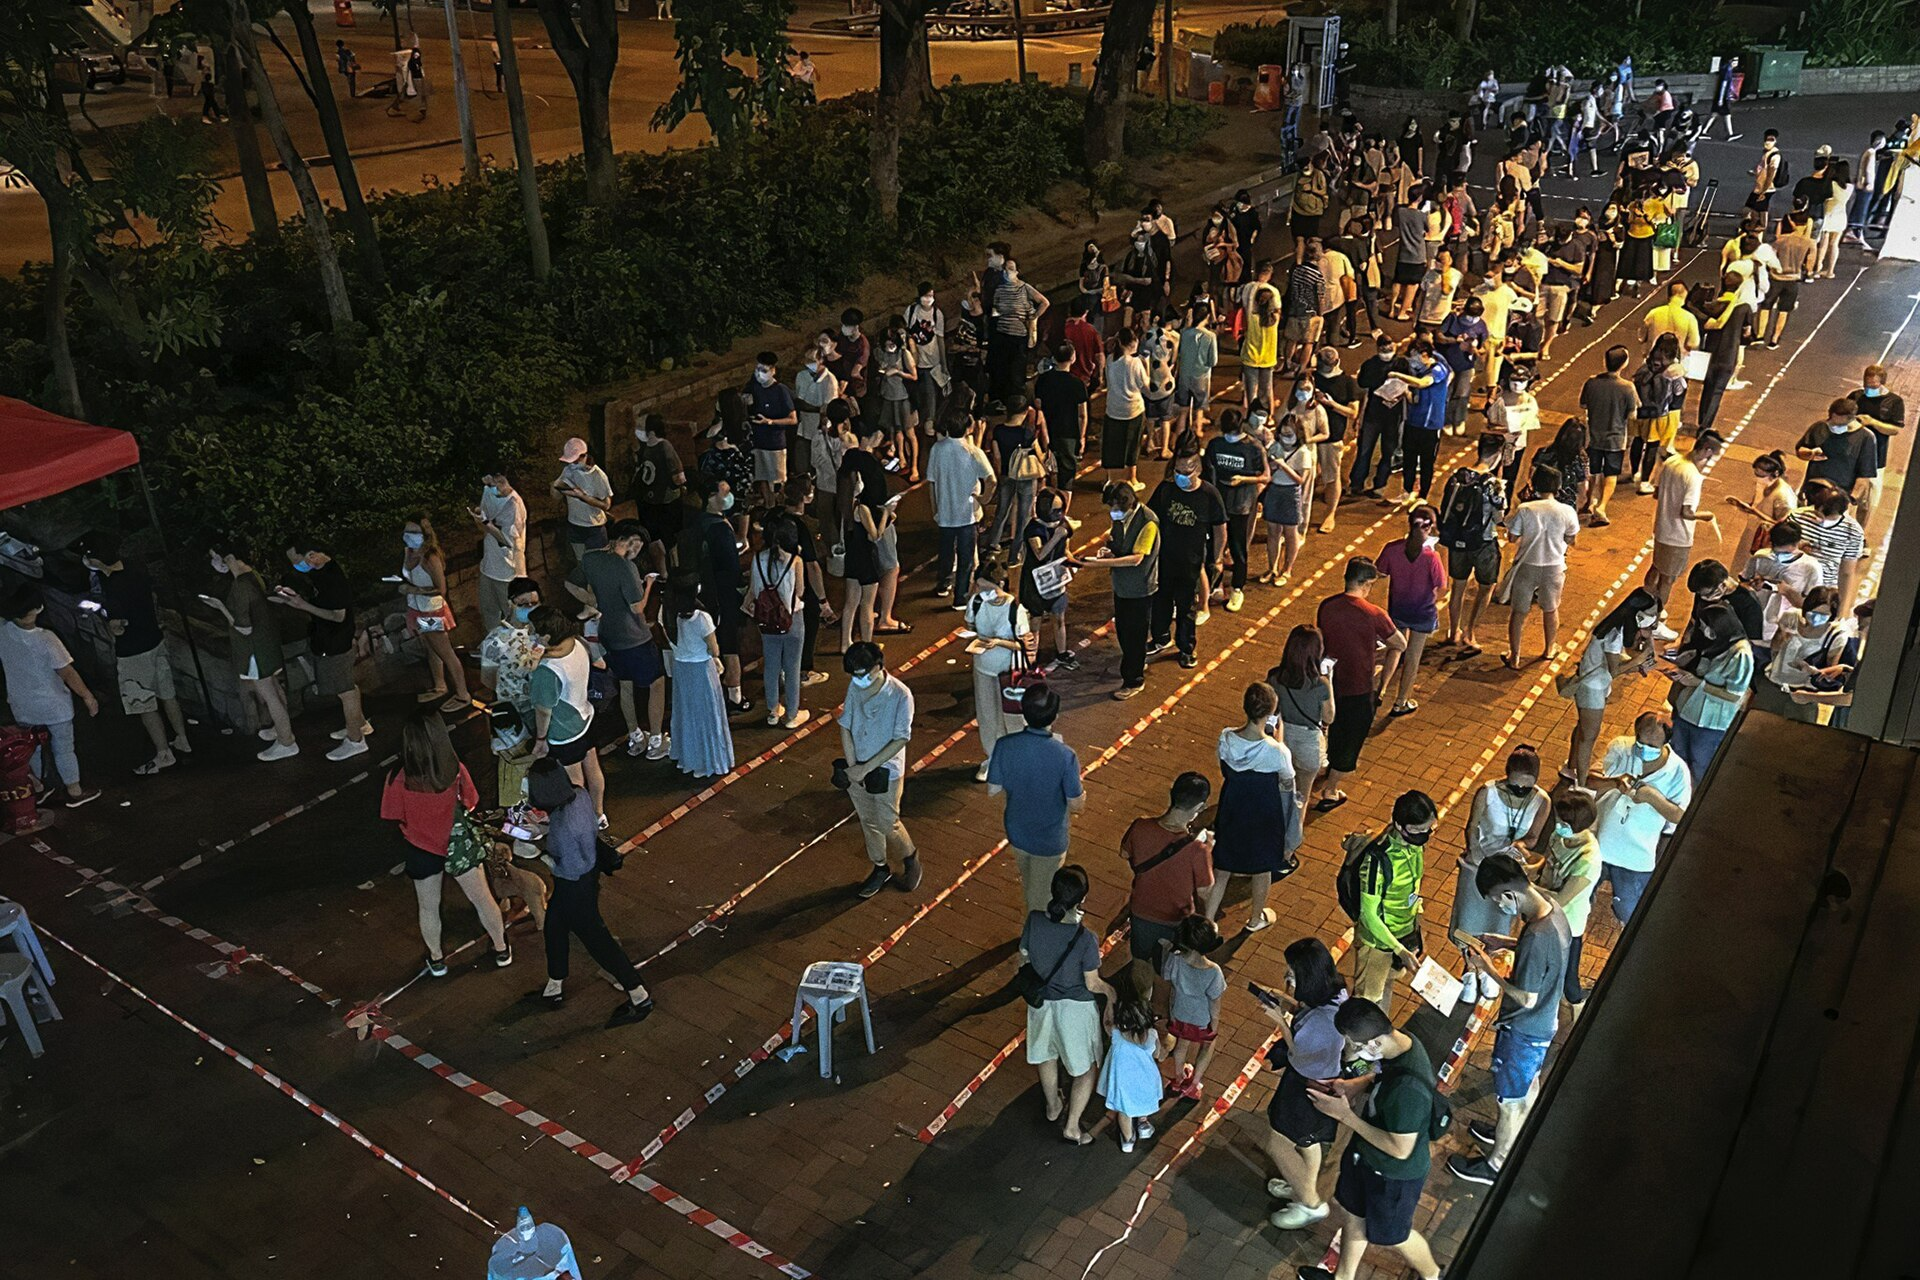
\includegraphics[width=0.5\linewidth]{assets/hongkong.png}

\end{frame}

\begin{frame}{Sorműveletek}

Queue() -- létrehoz egy üres sort

add(x : T) -- az x elemet a sor végére teszi

rem(): T -- a sor legelső elemét eltávolítja, és visszaadja

first(): T -- a sor legelső elemét visszaadja

isEmpty(): $\mathbb{B}$ -- visszaadja, hogy van-e elem a sorban


Egyelőre maradjunk ezen az absztrakciós szinten, ne vizsgáljuk hogyan implementálnánk.
    
\end{frame}

\begin{frame}{,,Dadogó'' szavak problémája}

Bemenetről érkezik egy szöveg és el kell dönteni, hogy a bemeneti szöveg ,,dadogós''-e vagy sem.

Példa: ``aa'', ``almaalma'', <> (üres szöveg is dadogósnak tekinthető)

Ötlet:

\begin{itemize}
    \item Olvassuk be a szöveget egy sorba.
    \item Ha a hossz páratlan, akkor nem ,,dadogós''.
    \item Ha páros, az egyik felét másoljuk egy másik sorba, majd hasonlítsuk össze.
\end{itemize}

\end{frame}

\begin{frame}[t]{,,Dadogó'' szavak problémája}

Bemenetről érkezik egy szöveg és el kell dönteni, hogy a bemeneti szöveg ,,dadogós''-e vagy sem.

\end{frame}

\begin{frame}[t]{Pascal-háromszög kiszámítása}

\[
\begin{array}{c}
       1 \\
     1 \quad 1 \\
   1 \quad 2 \quad 1 \\
 1 \quad 3 \quad 3 \quad 1
\end{array}
\]

Adott $k$ esetén számítsuk ki a $k$. sort.

Ne használjuk a direkt képletet: $\dfrac{k!}{i!\cdot(k-i)!}$

Dolgozzon az algoritmus sorról sorra, és használja ki, hogy minden szám a felette levő kettő összege.

\end{frame}

\begin{frame}[t]{Pascal-háromszög kiszámítása}

Bemenet: $k \in \mathbb{N}$ (az ennyiedik sort akarjuk kiszámítani)

\end{frame}

\fi

\end{document}
